\documentclass{tufte-handout}
\usepackage{CJKutf8}

%\geometry{showframe}% for debugging purposes -- displays the margins

%%%%%%%%%%%%%%%%%%%%%%%%%%%%%%%%%%%
% File: hw-preamble.tex
%%%%%%%%%%%%%%%%%%%%%%%%%%%%%%%%%%%

% Set fonts commands
\newcommand{\song}{\CJKfamily{song}} 
\newcommand{\hei}{\CJKfamily{hei}} 
\newcommand{\kai}{\CJKfamily{kai}} 
\newcommand{\fs}{\CJKfamily{fs}}

% colors
\newcommand{\red}[1]{\textcolor{red}{#1}}
\newcommand{\blue}[1]{\textcolor{blue}{#1}}
\newcommand{\teal}[1]{\textcolor{teal}{#1}}

% math
\newcommand{\set}[1]{\{#1\}}

% For math
\usepackage{amsmath}

% Define theorem-like environments
\usepackage[amsmath, thmmarks]{ntheorem}

\theoremstyle{break}
\theorembodyfont{\song}
\theoremseparator{}
\newtheorem*{problem}{Problem}

\theorempreskip{2.0\topsep}
\theoremheaderfont{\kai\bfseries}
\theoremseparator{:}
\newtheorem*{solution}{Solution}

\theoremstyle{break}
\theorempostwork{\bigskip\hrule}
\theoremsymbol{\ensuremath{\Box}}
\newtheorem*{proof}{Proof}

% algorithms
\usepackage[]{algorithm}
\usepackage[noend]{algpseudocode} % noend
% See [Adjust the indentation whithin the algorithmicx-package when a line is broken](https://tex.stackexchange.com/a/68540/23098)
\newcommand{\algparbox}[1]{\parbox[t]{\dimexpr\linewidth-\algorithmicindent}{#1\strut}}
\newcommand{\hStatex}[0]{\vspace{5pt}}
\makeatletter
\newlength{\trianglerightwidth}
\settowidth{\trianglerightwidth}{$\triangleright$~}
\algnewcommand{\LineComment}[1]{\Statex \hskip\ALG@thistlm \(\triangleright\) #1}
\algnewcommand{\LineCommentCont}[1]{\Statex \hskip\ALG@thistlm%
  \parbox[t]{\dimexpr\linewidth-\ALG@thistlm}{\hangindent=\trianglerightwidth \hangafter=1 \strut$\triangleright$ #1\strut}}
\makeatother

% For figures
% for fig with caption: #1: width/size; #2: fig file; #3: fig caption
\newcommand{\fig}[3]{
  \begin{figure}[htp]
    \centering
      \includegraphics[#1]{#2}
      \caption{#3}
  \end{figure}
}

% for fig without caption: #1: width/size; #2: fig file
\newcommand{\fignocaption}[2]{
  \begin{figure}[htp]
    \centering
    \includegraphics[#1]{#2}
  \end{figure}
}
\newcommand{\euclid}{\textsc{Euclid}}
\newcommand{\equal}{\textsc{Equal}}


\usepackage{amsmath}

% Set up the images/graphics package
\usepackage{graphicx}
\setkeys{Gin}{width=\linewidth,totalheight=\textheight,keepaspectratio}
\graphicspath{{graphics/}}

\title{2-1 The Correctness of Algorithms\thanks{Wish all your correctness proofs were \uppercase{correct}!}}
\author[hengxin]{Hengfeng Wei}
\date{13 March 2018}  % if the \date{} command is left out, the current date will be used

% The following package makes prettier tables.  We're all about the bling!
\usepackage{booktabs}

% The units package provides nice, non-stacked fractions and better spacing
% for units.
\usepackage{units}

% The fancyvrb package lets us customize the formatting of verbatim
% environments.  We use a slightly smaller font.
\usepackage{fancyvrb}
\fvset{fontsize=\normalsize}

% Small sections of multiple columns
\usepackage{multicol}

% Provides paragraphs of dummy text
\usepackage{lipsum}

% These commands are used to pretty-print LaTeX commands
\newcommand{\doccmd}[1]{\texttt{\textbackslash#1}}% command name -- adds backslash automatically
\newcommand{\docopt}[1]{\ensuremath{\langle}\textrm{\textit{#1}}\ensuremath{\rangle}}% optional command argument
\newcommand{\docarg}[1]{\textrm{\textit{#1}}}% (required) command argument
\newenvironment{docspec}{\begin{quote}\noindent}{\end{quote}}% command specification environment
\newcommand{\docenv}[1]{\textsf{#1}}% environment name
\newcommand{\docpkg}[1]{\texttt{#1}}% package name
\newcommand{\doccls}[1]{\texttt{#1}}% document class name
\newcommand{\docclsopt}[1]{\texttt{#1}}% document class option name

\begin{document}
\begin{CJK*}{UTF8}{gbsn}

\maketitle% this prints the handout title, author, and date

\begin{abstract}
\noindent We show how to prove the correctness of two algorithms:
One is an iterative algorithm called $\equal(S_1, S_2)$ for comparing two strings.
The other is the classic recursive Euclid algorithm for computing the greatest common divisor (gcd) of two natural numbers.
\end{abstract}

%\printclassoptions

\section{DH Problem 5.9: $\equal(S_1, S_2)$}  \label{section:problem-5.9}
  Construct a function $\equal(S_1, S_2)$ that tests whether the strings $X$ and $Y$ are equal.
  It should return true or false accordingly.

  You may use the following operations:
  \begin{itemize}
    \item $\texttt{head}(X)$
    \item $\texttt{tail}(X)$
    \item $\texttt{last}(X)$
    \item $\texttt{all-but-last}(X)$
    \item $\texttt{eq}(s,t)$
  \end{itemize}

\subsection{Solution}


The algorithm $\equal(S_1, S_2)$ is shown in Algorithm~\ref{alg:equal},
with appropriate assertions attached.

The partial correctness of $\equal$ can be denoted as
\marginnote{Using the notations of Hoare logic developed by Tony Hoare. \cite{Hoare:CACM69}}

\begin{marginfigure}%
  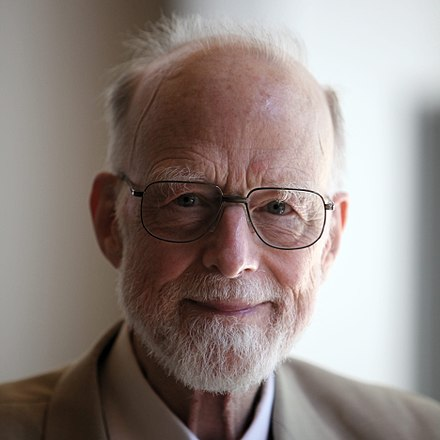
\includegraphics[width=0.60\linewidth]{figs/tony-hoare}
  \label{fig:hoare}
\end{marginfigure}
\[
  P \;\set{\equal}\; Q,
\]
meaning that if the input satisfies the precondition $P$, 
then after $\equal$ the postcondition $Q$ must hold.
To this end, we show that:

% file: algs/equal.tex

\begin{algorithm}[t]
  \caption{Comparing two strings.}
  \label{alg:equal}
  \begin{algorithmic}[1]
    \Procedure{Equal}{$S_1,S_2$} 
      \LineComment{\teal{$P: S_1, S_2$ are strings}}
      \State $X \gets S_1$
      \State $Y \gets S_2$
      \State $E \gets \top$
      \hStatex

      \LineComment{\teal{(1) $I: S_1 = S_2 \iff X = Y \land E = \top$}}
      \While{$X \neq \epsilon \land Y \neq \epsilon \land E = \top$}
	\If{$\texttt{eq}(\texttt{head}(X), \texttt{head}(Y))$}
	  \State $X \gets \texttt{tail}(X)$
	  \State $Y \gets \texttt{tail}(Y)$
	\Else
	  \State $E \gets \bot$
	\EndIf
      \EndWhile

      \hStatex
      \LineComment{\teal{(2) $S_1 = S_2 \iff (X = \epsilon \land Y = \epsilon) \land E = \top$}}
      \If{$\lnot (X = \epsilon \land Y = \epsilon)$}
        \State $E \gets \bot$
	\LineComment{\teal{(3.1) $S_1 \neq S_2 \land E = \bot$}}
      \Else
	\State \texttt{DoNothing}  \Comment{Just for inserting an assertion here.}
	\LineComment{\teal{(3.2) $S_1 = S_2 \iff E = \top$}}
      \EndIf

      \hStatex
      \LineComment{\teal{(4) $Q: S_1 = S_2 \iff E = \top$}}
      \State \Return $E$
    \EndProcedure
  \end{algorithmic}
\end{algorithm}



\begin{enumerate}[(i)]
  \item $I$ is a loop invariant.
  \item (2) is an invariant.
    \[
      I \land \lnot (X \neq \epsilon \land Y \neq \epsilon \land E = \top) \implies (2)
    \]
  \item (3.1) is an invariant
  \item (3.2) is an invariant
  \item $Q$ is an invariant
\end{enumerate}

\section{Extra Problem: $\euclid(m, n)$}  \label{section:euclid}

Prove the following recursive Euclid algorithm for 
computing the greatest common divisor (gcd) of two natural numbers are totally correct.

\begin{marginfigure}%
  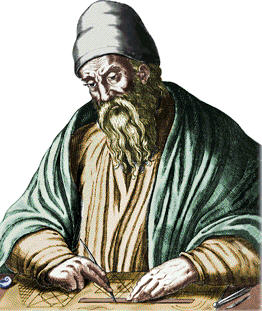
\includegraphics[width=0.60\linewidth]{figs/euclid}
  \label{fig:euclid}
\end{marginfigure}

% file: problems/euclid.tex

\section{Extra Problem: $\euclid(m, n)$}  \label{section:euclid}

Prove the recursive Euclid algorithm as shown in Algorithm~\ref{alg:euclid} for 
computing the greatest common divisor (gcd) of two natural numbers are totally correct.

\begin{marginfigure}%
  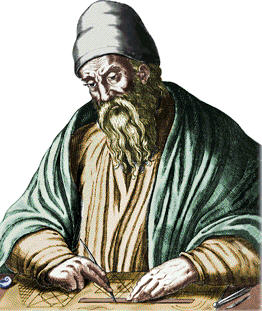
\includegraphics[width=0.60\linewidth]{figs/euclid}
  \label{fig:euclid}
\end{marginfigure}

% file: problems/euclid.tex

\section{Extra Problem: $\euclid(m, n)$}  \label{section:euclid}

Prove the recursive Euclid algorithm as shown in Algorithm~\ref{alg:euclid} for 
computing the greatest common divisor (gcd) of two natural numbers are totally correct.

\begin{marginfigure}%
  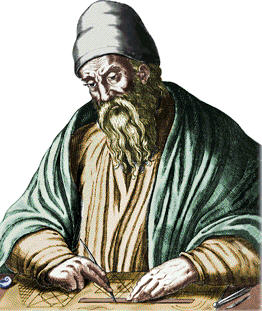
\includegraphics[width=0.60\linewidth]{figs/euclid}
  \label{fig:euclid}
\end{marginfigure}

% file: problems/euclid.tex

\section{Extra Problem: $\euclid(m, n)$}  \label{section:euclid}

Prove the recursive Euclid algorithm as shown in Algorithm~\ref{alg:euclid} for 
computing the greatest common divisor (gcd) of two natural numbers are totally correct.

\begin{marginfigure}%
  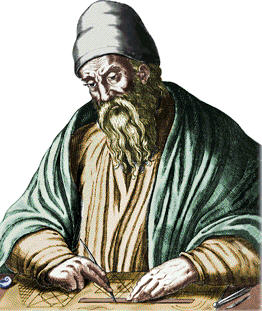
\includegraphics[width=0.60\linewidth]{figs/euclid}
  \label{fig:euclid}
\end{marginfigure}

\input{algs/euclid}

\subsection{Proof}

\marginnote{Also pay attention to the way how to write a mathematical induction proof.}

We prove the partial correctness of \euclid{} by strong mathematical induction on $n$,
with $m$ any fixed natural number.

\begin{description}
  \item[Basis:] $n = 0$. We have that
    \marginnote{Make sure you understand each of these three ``='''s:
      \begin{enumerate}[(1)]
	\item By $n = 0$;
	\item By the property of $\gcd$;
	\item By the \euclid{} algorithm.
      \end{enumerate}
    }
    \[
      \gcd(m,n) = \gcd(m,0) = m = \euclid(m,0).
    \]
  \item[Inductive Hypothesis:]
    Suppose that $n \ge 1$ and
    \[
      \gcd(m, k) = \euclid(m, k), \;\forall 0 \le k \le n - 1.
    \]
  \item[Inductive Step:]
    We need to prove that ($n \ge 1$)
    \[
      \gcd(m, n) = \euclid(m, n).
    \]

    According to \euclid{}, we have
    \[
      \euclid(m,n) = \euclid(n, m \bmod n).
    \]
    Since $(m \bmod n) < n$, by the inductive hypothesis, we have
    \[
      \euclid(n, m \bmod n) = \gcd(n, m \bmod n).
    \]
    Therefore, it suffices to prove that
    \[
      \boxed{\gcd(m,n) = \gcd(n, m \bmod n).}
    \]
    For notational convenience, we denote
    \[
      d = \gcd(m,n), \quad d' = \gcd(n, m \bmod n).
    \]
    Because $d, d' \ge 0$, it is sufficient to obtain $d = d'$
    by showing that $d \mid d'$ and $d' \mid d$:

    \begin{itemize}
      \item $d \mid d'$.
      \item $d' \mid d$.
    \end{itemize}
\end{description}


\subsection{Proof}

\marginnote{Also pay attention to the way how to write a mathematical induction proof.}

We prove the partial correctness of \euclid{} by strong mathematical induction on $n$,
with $m$ any fixed natural number.

\begin{description}
  \item[Basis:] $n = 0$. We have that
    \marginnote{Make sure you understand each of these three ``='''s:
      \begin{enumerate}[(1)]
	\item By $n = 0$;
	\item By the property of $\gcd$;
	\item By the \euclid{} algorithm.
      \end{enumerate}
    }
    \[
      \gcd(m,n) = \gcd(m,0) = m = \euclid(m,0).
    \]
  \item[Inductive Hypothesis:]
    Suppose that $n \ge 1$ and
    \[
      \gcd(m, k) = \euclid(m, k), \;\forall 0 \le k \le n - 1.
    \]
  \item[Inductive Step:]
    We need to prove that ($n \ge 1$)
    \[
      \gcd(m, n) = \euclid(m, n).
    \]

    According to \euclid{}, we have
    \[
      \euclid(m,n) = \euclid(n, m \bmod n).
    \]
    Since $(m \bmod n) < n$, by the inductive hypothesis, we have
    \[
      \euclid(n, m \bmod n) = \gcd(n, m \bmod n).
    \]
    Therefore, it suffices to prove that
    \[
      \boxed{\gcd(m,n) = \gcd(n, m \bmod n).}
    \]
    For notational convenience, we denote
    \[
      d = \gcd(m,n), \quad d' = \gcd(n, m \bmod n).
    \]
    Because $d, d' \ge 0$, it is sufficient to obtain $d = d'$
    by showing that $d \mid d'$ and $d' \mid d$:

    \begin{itemize}
      \item $d \mid d'$.
      \item $d' \mid d$.
    \end{itemize}
\end{description}


\subsection{Proof}

\marginnote{Also pay attention to the way how to write a mathematical induction proof.}

We prove the partial correctness of \euclid{} by strong mathematical induction on $n$,
with $m$ any fixed natural number.

\begin{description}
  \item[Basis:] $n = 0$. We have that
    \marginnote{Make sure you understand each of these three ``='''s:
      \begin{enumerate}[(1)]
	\item By $n = 0$;
	\item By the property of $\gcd$;
	\item By the \euclid{} algorithm.
      \end{enumerate}
    }
    \[
      \gcd(m,n) = \gcd(m,0) = m = \euclid(m,0).
    \]
  \item[Inductive Hypothesis:]
    Suppose that $n \ge 1$ and
    \[
      \gcd(m, k) = \euclid(m, k), \;\forall 0 \le k \le n - 1.
    \]
  \item[Inductive Step:]
    We need to prove that ($n \ge 1$)
    \[
      \gcd(m, n) = \euclid(m, n).
    \]

    According to \euclid{}, we have
    \[
      \euclid(m,n) = \euclid(n, m \bmod n).
    \]
    Since $(m \bmod n) < n$, by the inductive hypothesis, we have
    \[
      \euclid(n, m \bmod n) = \gcd(n, m \bmod n).
    \]
    Therefore, it suffices to prove that
    \[
      \boxed{\gcd(m,n) = \gcd(n, m \bmod n).}
    \]
    For notational convenience, we denote
    \[
      d = \gcd(m,n), \quad d' = \gcd(n, m \bmod n).
    \]
    Because $d, d' \ge 0$, it is sufficient to obtain $d = d'$
    by showing that $d \mid d'$ and $d' \mid d$:

    \begin{itemize}
      \item $d \mid d'$.
      \item $d' \mid d$.
    \end{itemize}
\end{description}


\subsection{Proof}

\marginnote{Also pay attention to the way how to write a mathematical induction proof.}

We prove the partial correctness of \euclid{} by strong mathematical induction on $n$,
with $m$ any fixed natural number.

\begin{description}
  \item[Basis:] $n = 0$. We have that
    \marginnote{Make sure you understand each of these three ``='''s:
      \begin{enumerate}[(1)]
	\item By $n = 0$;
	\item By the property of $\gcd$;
	\item By the \euclid{} algorithm.
      \end{enumerate}
    }
    \[
      \gcd(m,n) = \gcd(m,0) = m = \euclid(m,0).
    \]
  \item[Inductive Hypothesis:]
    Suppose that $n \ge 1$ and
    \[
      \gcd(m, k) = \euclid(m, k), \;\forall 0 \le k \le n - 1.
    \]
  \item[Inductive Step:]
    We need to prove that ($n \ge 1$)
    \[
      \gcd(m, n) = \euclid(m, n).
    \]

    According to \euclid{}, we have
    \[
      \euclid(m,n) = \euclid(n, m \bmod n).
    \]
    Since $(m \bmod n) < n$, by the inductive hypothesis, we have
    \[
      \euclid(n, m \bmod n) = \gcd(n, m \bmod n).
    \]
    Therefore, it suffices to prove that
    \[
      \boxed{\gcd(m,n) = \gcd(n, m \bmod n).}
    \]
    For notational convenience, we denote
    \[
      d = \gcd(m,n), \quad d' = \gcd(n, m \bmod n).
    \]
    Because $d, d' \ge 0$, it is sufficient to obtain $d = d'$
    by showing that $d \mid d'$ and $d' \mid d$:

    \begin{itemize}
      \item $d \mid d'$.
      \item $d' \mid d$.
    \end{itemize}
\end{description}

\bibliography{2-1-correctness}
\bibliographystyle{plainnat}

\end{CJK*}
\end{document}